% ----------------------------------------------------
% DAB Standard
% ----------------------------------------------------
\documentclass[class=report,11pt,crop=false]{standalone}
\input{../Style/ChapterStyle.tex}
\makenoidxglossaries

\newacronym{radar}{RADAR}{Radio Detection and Ranging}
\newacronym{dab}{DAB}{Digital Audio Broadcasting}
\newacronym{fm}{FM}{Frequency Modulation}
\newacronym{am}{AM}{Amplitude Modulation}
\newacronym{fdm}{FDM}{Frequency Division Multiplexing}
\newacronym{ofdm}{OFDM}{Orthogonal Frequency Division Multiplexing}
\newacronym{cofdm}{COFDM}{Coded Orthogonal Frequency Division Multiplexing}
\newacronym{dvbt2}{DVB–T2}{Digital Video Broadcasting — Second Generation Terrestrial}
\newacronym{em}{EM}{electromagnetic}
\newacronym{icasa}{ICASA}{Independent Communications Authority of South Africa}
\newacronym{ioo}{IOO}{Illuminators of Opportunity}
\newacronym{pr}{PR}{Passive Radar}
\newacronym{qpsk}{QPSK}{Quadrature Phase-Shift Keying}
\newacronym{dqpsk}{DQPSK}{Differential~Quadrature~Phase-Shift~Keying}
\newacronym{etsi}{ETSI}{European Telecommunications Standards Institute}
\newacronym{psk}{PSK}{Phase Shift Keying}
\newacronym{ask}{ASK}{Amplitude-Shift Keying}
\newacronym{fsk}{FSK}{Frequency-Shift Keying}
\newacronym{iq}{IQ}{In-phase and Quadrature}
\newacronym{ns}{NS}{Null Symbol}
\newacronym{prs}{PRS}{Phase Reference Symbol}
\newacronym{fic}{FIC}{Fast Information Channel}
\newacronym{msc}{MSC}{Main Service Channel}
\newacronym{dft}{DFT}{Discrete Fourier Transform}
\newacronym{idft}{IDFT}{Inverse Discrete Fourier Transform}
\newacronym{fft}{FFT}{Fast Fourier Transform}
\newacronym{ifft}{IFFT}{Inverse Fast Fourier Transform}
\newacronym{fec}{FEC}{Forward Error Correction}
\newacronym{ard}{ARD}{Amplitude-Range-Doppler}
\newacronym{snr}{SNR}{Signal-to-Noise Ratio}
\newacronym{isi}{ISI}{Intersymbol Interference}
\newacronym{mcm}{MCM}{Multicarrier Modulation}
\begin{document}
\ifstandalone
\tableofcontents
\fi
% ----------------------------------------------------
\chapter{Digital Audio Broadcasting: Standard}
\epigraph{Where the waters do agree, it is quite wonderful the relief they give.}%
{\emph{---Jane Austen, Emma}}
% ----------------------------------------------------

\section{Overview}
This chapter aims to outline the key components of the \gls{dab} standard, as prescribed by the \gls{etsi} in~\cite{dabstandard}. This begins with a discussion on \gls{cofdm} and \gls{dqpsk}, each of which is fundamental to \gls{dab}. Thereafter, the structure of a \gls{dab} frame will be mentioned, with special highlights made to the null and phase-reference symbols. Note, however, that since this report focuses on \gls{dab} signals within the context of \gls{pr}, it is unnecessary for a complete and thorough description of the \gls{dab} format---in fact, many simplifications can be made. The \gls{dab}-based \gls{pr} chain need not dive into the specifics of the source audio coding, and so on.

\section{Coded Orthogonal Frequency Division Multiplexing}
In 1966, Robert W. Chang published an incredibly important paper~\cite{Chang1966}, outlining the idea of \gls{ofdm}.

\subsection{Motivation}
Suppose one wanted to transmit a set of symbols, \(\mathcal{D}\), using an amplitude modulation scheme, for the sake of the example. There are, in essence, two approaches to do this. The first, which is markedly simpler, is a serial approach: simply to modulate a carrier wave with successive elements of \(\mathcal{D}\). Alternatively, one could take a parallel approach. That is, to split \(\mathcal{D}\) into \(n\) subsets, and then use these subsets to modulate \(n\) independent carriers respectively. Figure~\ref{fig:carrier-illustration} illustrates these situations with two simplified spectrograms---for the sake of clarity, the frequency components are shown to be perfectly impulsive. Here, each carrier wave's amplitude is modulated with various symbol values, where each symbol lasts for a fixed period in time.

Phase shift keying modulation, which is explained properly in section~\ref{sect:dab-std_psk}.

\begin{figure}[htbp]
    \centering
    \begin{subfigure}[t]{0.48\textwidth}
        \centering
        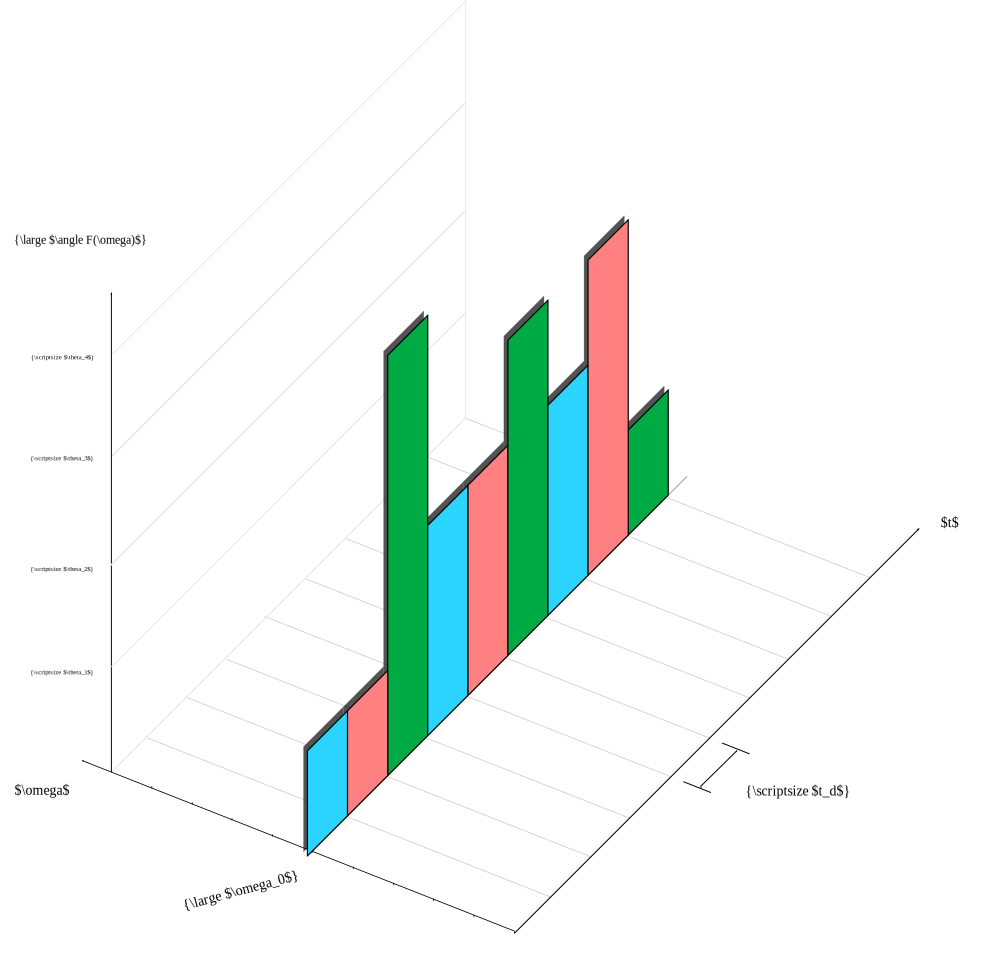
\includegraphics[width=0.95\linewidth]{serial-carrier.pdf}
        \caption{Single carrier with a higher data-rate}
        \label{fig:serial-carrier}
    \end{subfigure}%
    ~ 
    \begin{subfigure}[t]{0.48\textwidth}
        \centering
        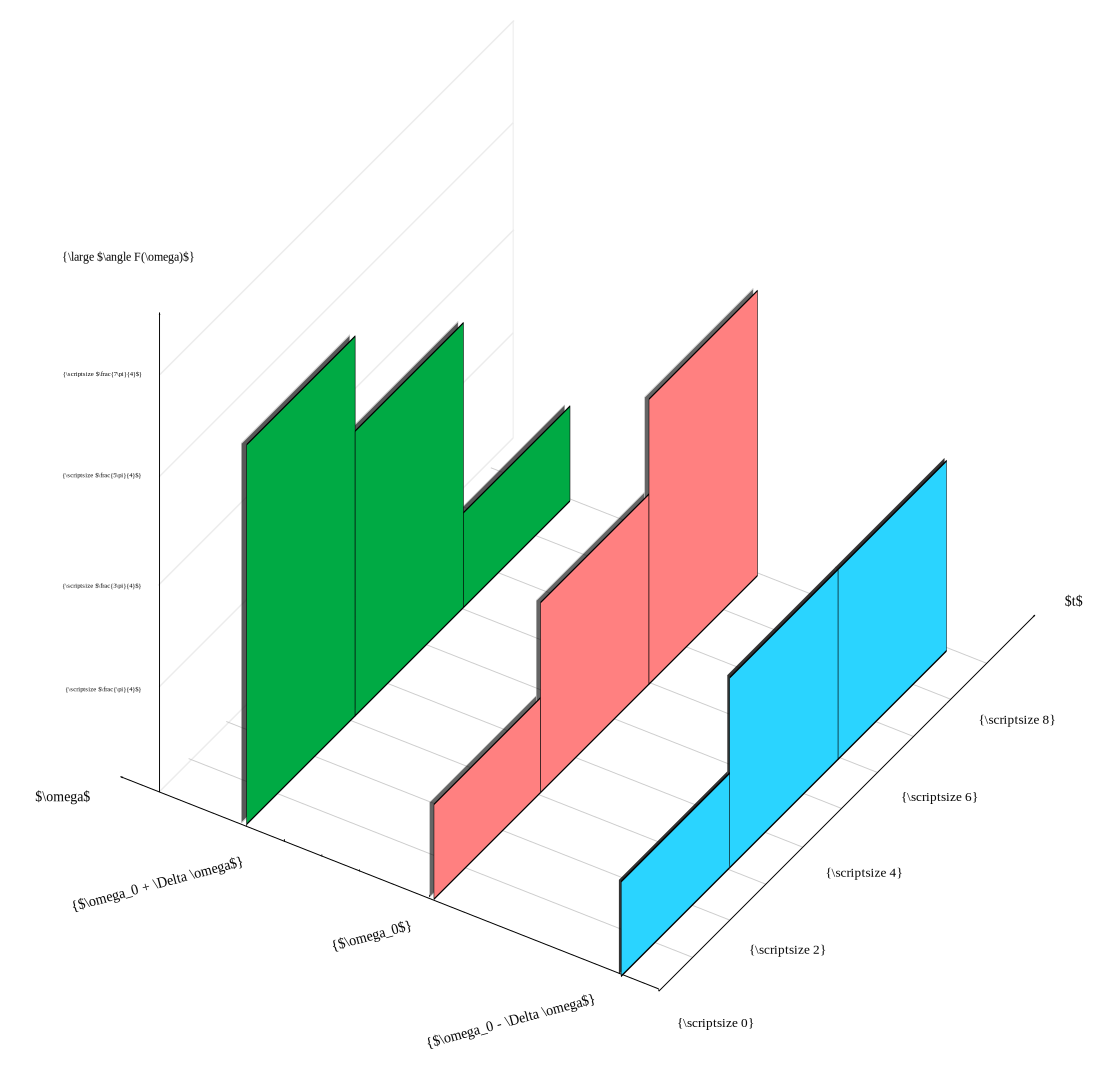
\includegraphics[width=0.9\linewidth]{parallel-carrier.pdf}
        \caption{Multiple carriers with a lower data-rate}
        \label{fig:parallel-carrier}
    \end{subfigure}
    \caption{}
    \label{fig:carrier-illustration}
\end{figure}

Figure~\ref{fig:serial-carrier} shows the serial case, where all 9 symbols are successively modulated on the carrier wave with a frequency of \(\omega_0\). Figure~\ref{fig:parallel-carrier}, on the other hand, shows the parallel case, with the 9 symbols split into 3 separate groups, respectively modulating carriers with frequencies of \((\omega_0 - \Delta \omega)\), \(\omega_0\), and \((\omega_0 + \Delta \omega)\). Notice the symbol period for the latter situation is 3 times longer than that of the former.

While the serial scheme is simpler, the parallel scheme has two important advantages.

Multipath, inter-symbol interference

Frequency selective fading

\subsection{Frequency Division Multiplexing}
The illustration from figure~\ref{fig:carrier-illustration} was an example of \gls{fdm}, where the frequency domain is divided---i.e. multiplexed---into separate regions, each carrying independent information. There is one caveat with the previous example, however. The frequency components, as shown, were assumed to be impulsive. This implies that adjacent carriers could be infinitely close to each other without any crosstalk---that is, interference between the carriers. Unfortunately, this cannot be the case.

To understand why, consider a carrier wave, \(f(t)\), which has a frequency of \(\omega_0\), and is recorded over a period of \(T\) seconds. Notice that this is equivalent to multiplying \(f(t)\) by a windowing function, \(w(t)\), with a width of \(T\). Figure~\ref{fig:sampling-sine} depicts this, where a simple rectangular pulse is used as the windowing function. Note, however, that more complex windowing functions can be used, and the point will remain. The resulting windowed carrier wave is notated as \(f_T(t)\).

\begin{figure}
    \centering
    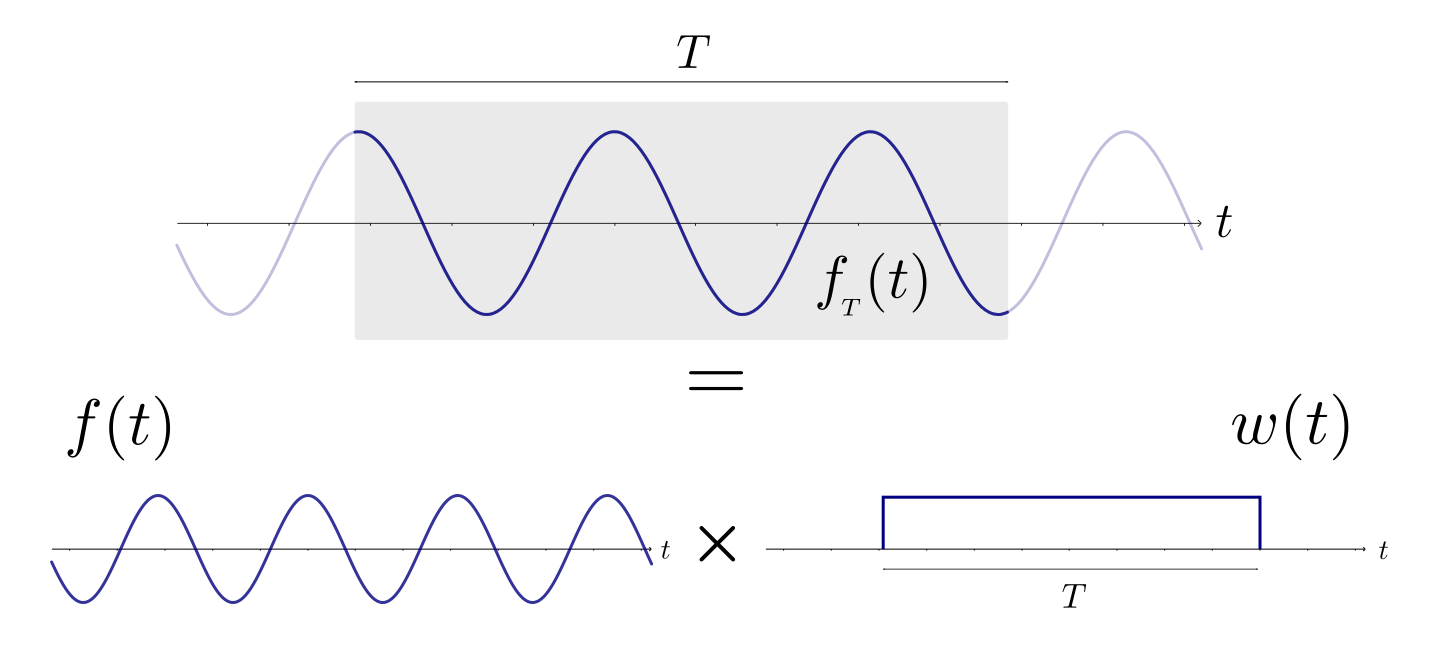
\includegraphics[width=\linewidth]{sampling-sine.pdf}
    \caption{Depiction of sampling as a multiplication with a finite window function}
    \label{fig:sampling-sine}
\end{figure}

Consider now the impact of windowing as viewed in the frequency domain. The original carrier wave, \(f(t)\), which theoretically spans over all time, is perfectly impulsive. However, multiplication with the windowing function in time is equivalent to convolution with the window's spectrum in frequency. The exact details of this spectrum depend on the windowing function used, but for a simple rectangular function,
\begin{equation}
    w(t) = \textrm{rect}\Big(\frac{t}{T}\Big) \xLeftrightarrow{\quad\mathcal{F}\quad} W(\omega) = \text{Sa}()
\end{equation}


\begin{figure}
    \centering
    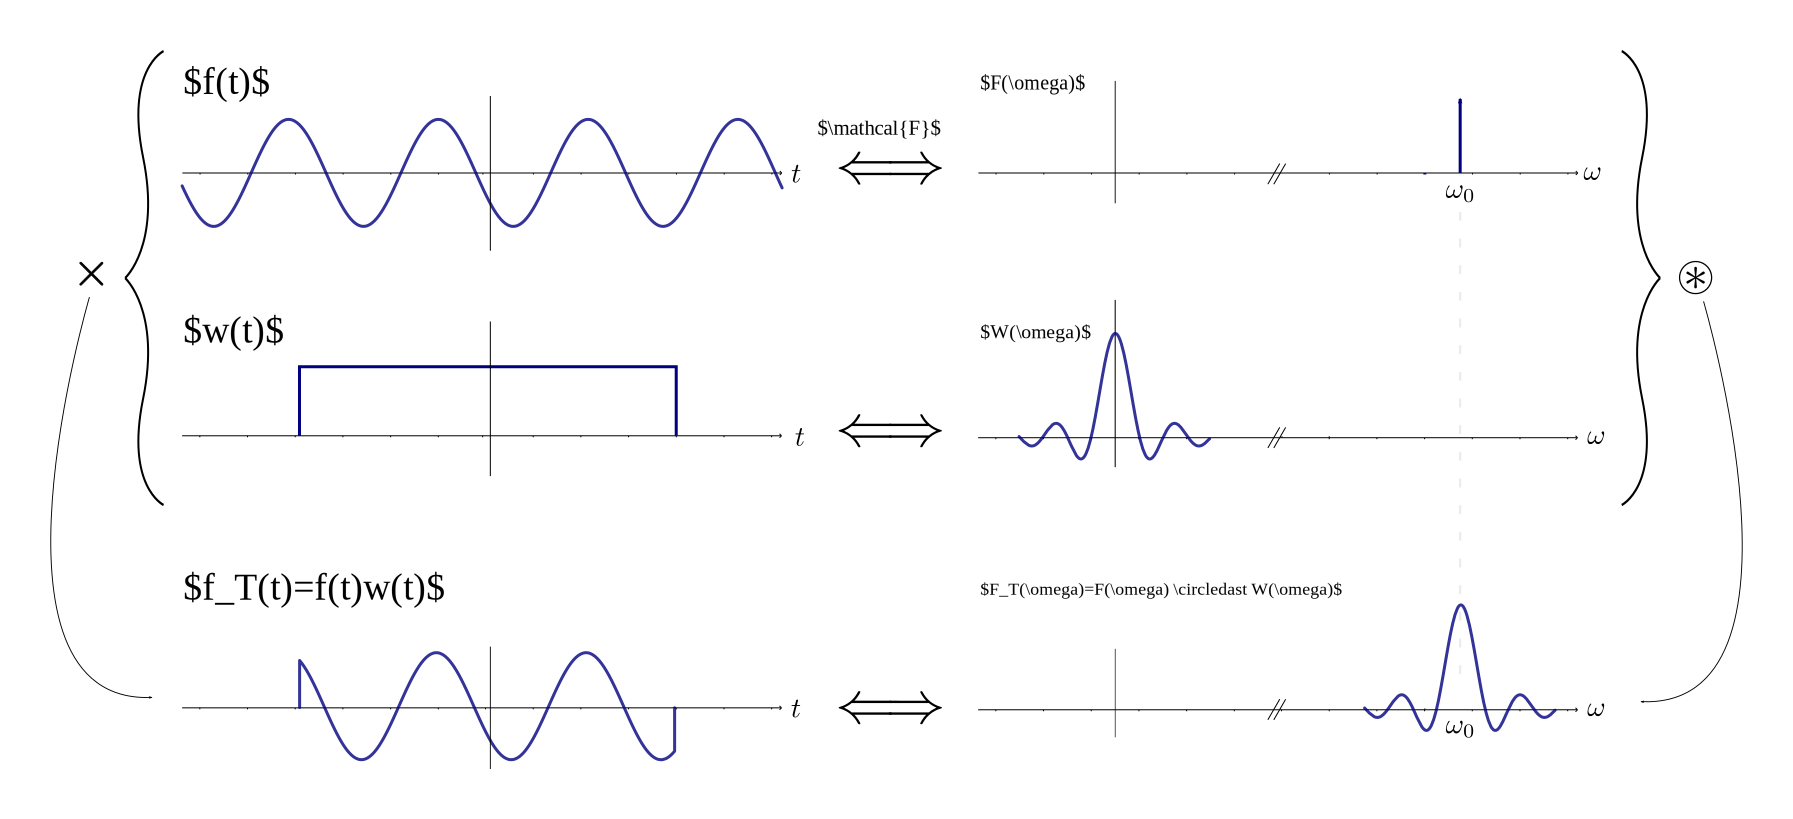
\includegraphics[width=\linewidth]{sampling-sine-freq.pdf}
    \caption{Effect of windowing on spectrum}
    \label{fig:sampling-sine-freq}
\end{figure}

Instead, each carrier has an associated spectrum, and this spectrum influences the ability for one to demodulate the other carriers.

How, then, does that influence the ability to perform \gls{fdm}?

Suppose one has three carriers, each with a \(\textrm{Sa}(\omega) = \frac{\sin \omega}{\omega}\) spectrum. If the centre frequencies of these carriers are sufficiently distant from the others, there will be negligible interference from one spectrum's sidelobes to another spectrum's mainlobe. This is seen in figure~\ref{fig:three-sincs-good-distance}.


\begin{figure}
    \centering
    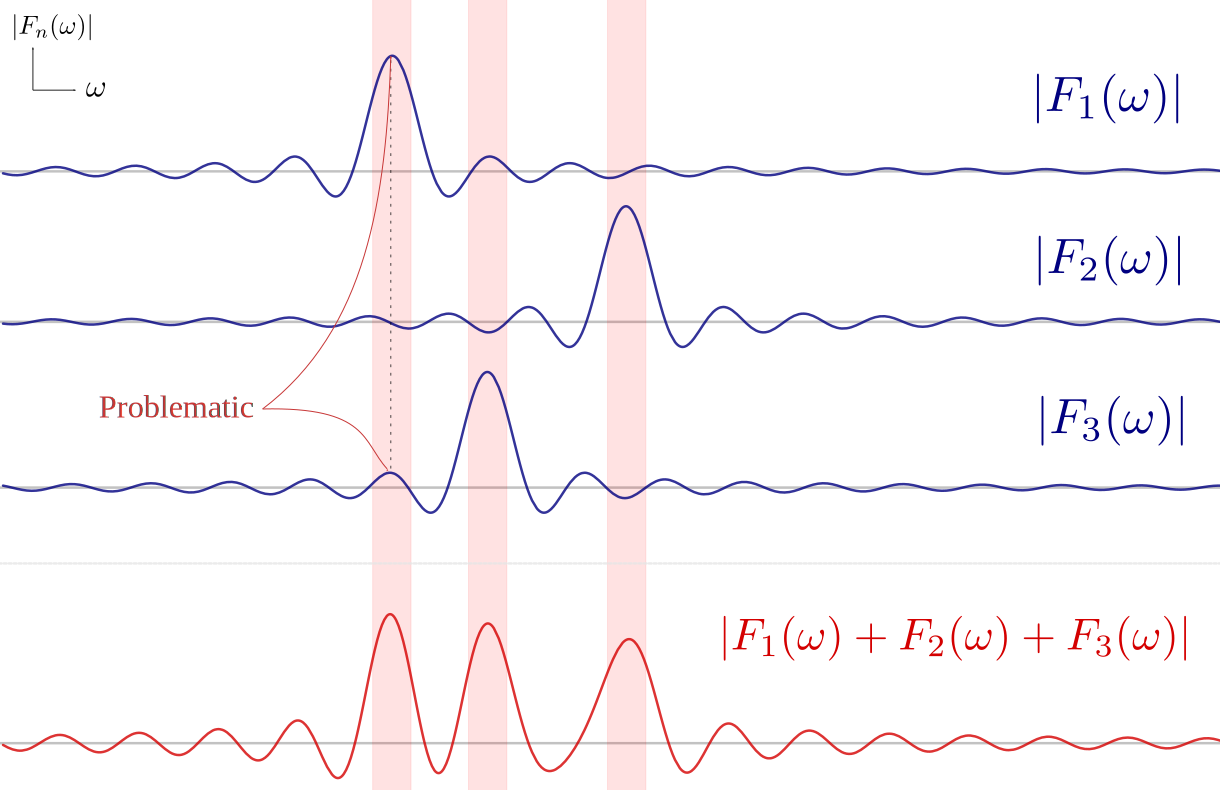
\includegraphics[width=\linewidth]{three-sincs-bad-distance.pdf}
    \caption{Three spectra spaced insufficiently far away from each other}
    \label{fig:three-sincs-bad-distance}
\end{figure}

\begin{figure}
    \centering
    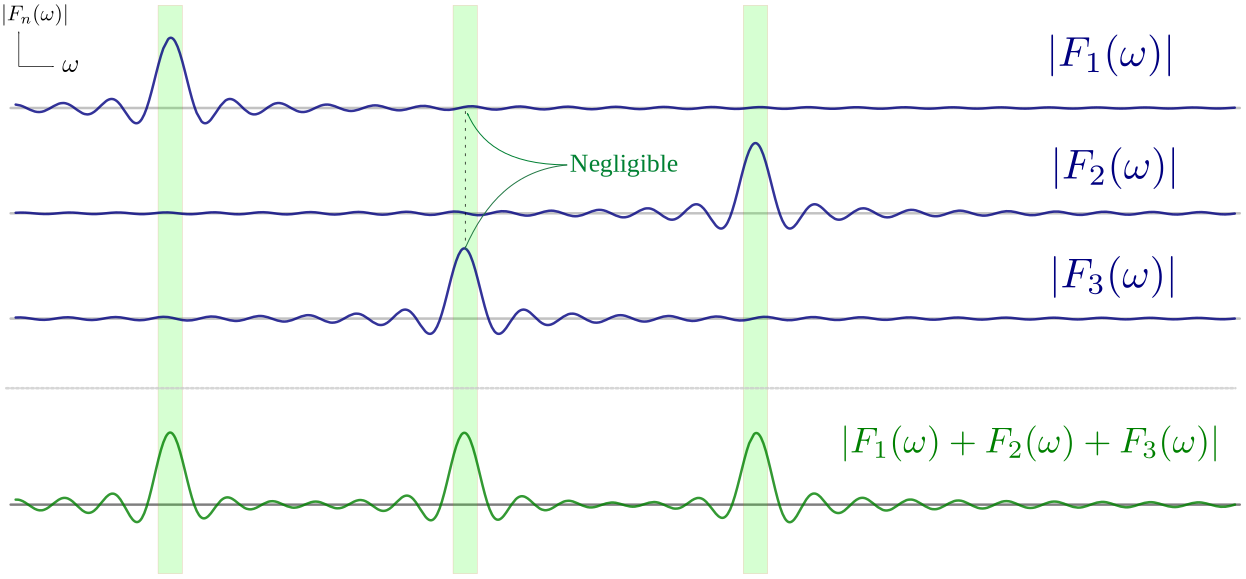
\includegraphics[width=\linewidth]{three-sincs-good-distance.pdf}
    \caption{Three spectra spaced sufficiently far away from each other}
    \label{fig:three-sincs-good-distance}
\end{figure}



\subsection{Orthogonal Carriers}


\begin{figure}
    \centering
    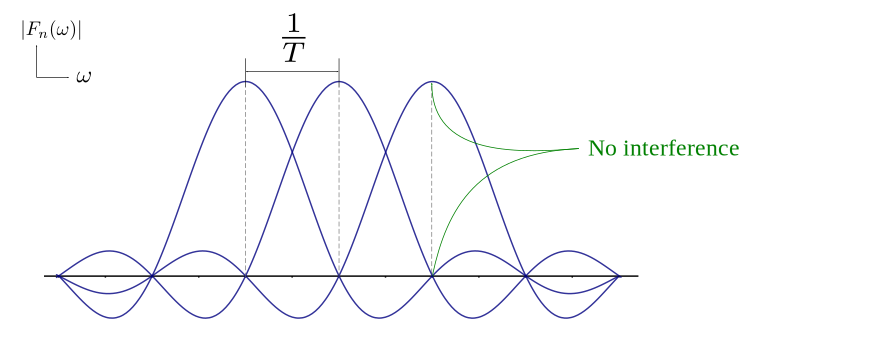
\includegraphics[width=\linewidth]{ofdm-three-sincs.pdf}
    \caption{Three spectra arranged orthogonally}
    \label{fig:ofdm-three-sincs}
\end{figure}


\subsection{Time \& Frequency Interleaving}


\subsection{Forward Error Correction}



\section{Phase Shift Keying \label{sect:dab-std_psk}}
\subsection{Motivation}
\subsection{Quadrature Phase Shift Keying}
\subsection{Differential Quadrature Phase Shift Keying}


\section{Transmission Frame}


\subsection{Overview}


\subsection{Null Symbol}


\subsection{Phase Reference Symbol}


\subsection{Data-carrying Symbols}


\subsection{Guard Intervals}



\section{Summary}


% ----------------------------------------------------
\ifstandalone
\bibliography{../Bibliography/References.bib}
\printnoidxglossary[type=\acronymtype,nonumberlist]
\fi
\end{document}
% ----------------------------------------------------